


\begin{frame}{Contents}
  \begin{center}
   \Large Part 4: ViennaMath
  \end{center}
\end{frame}

\begin{frame}{Simulation Flow}
  \begin{center}
   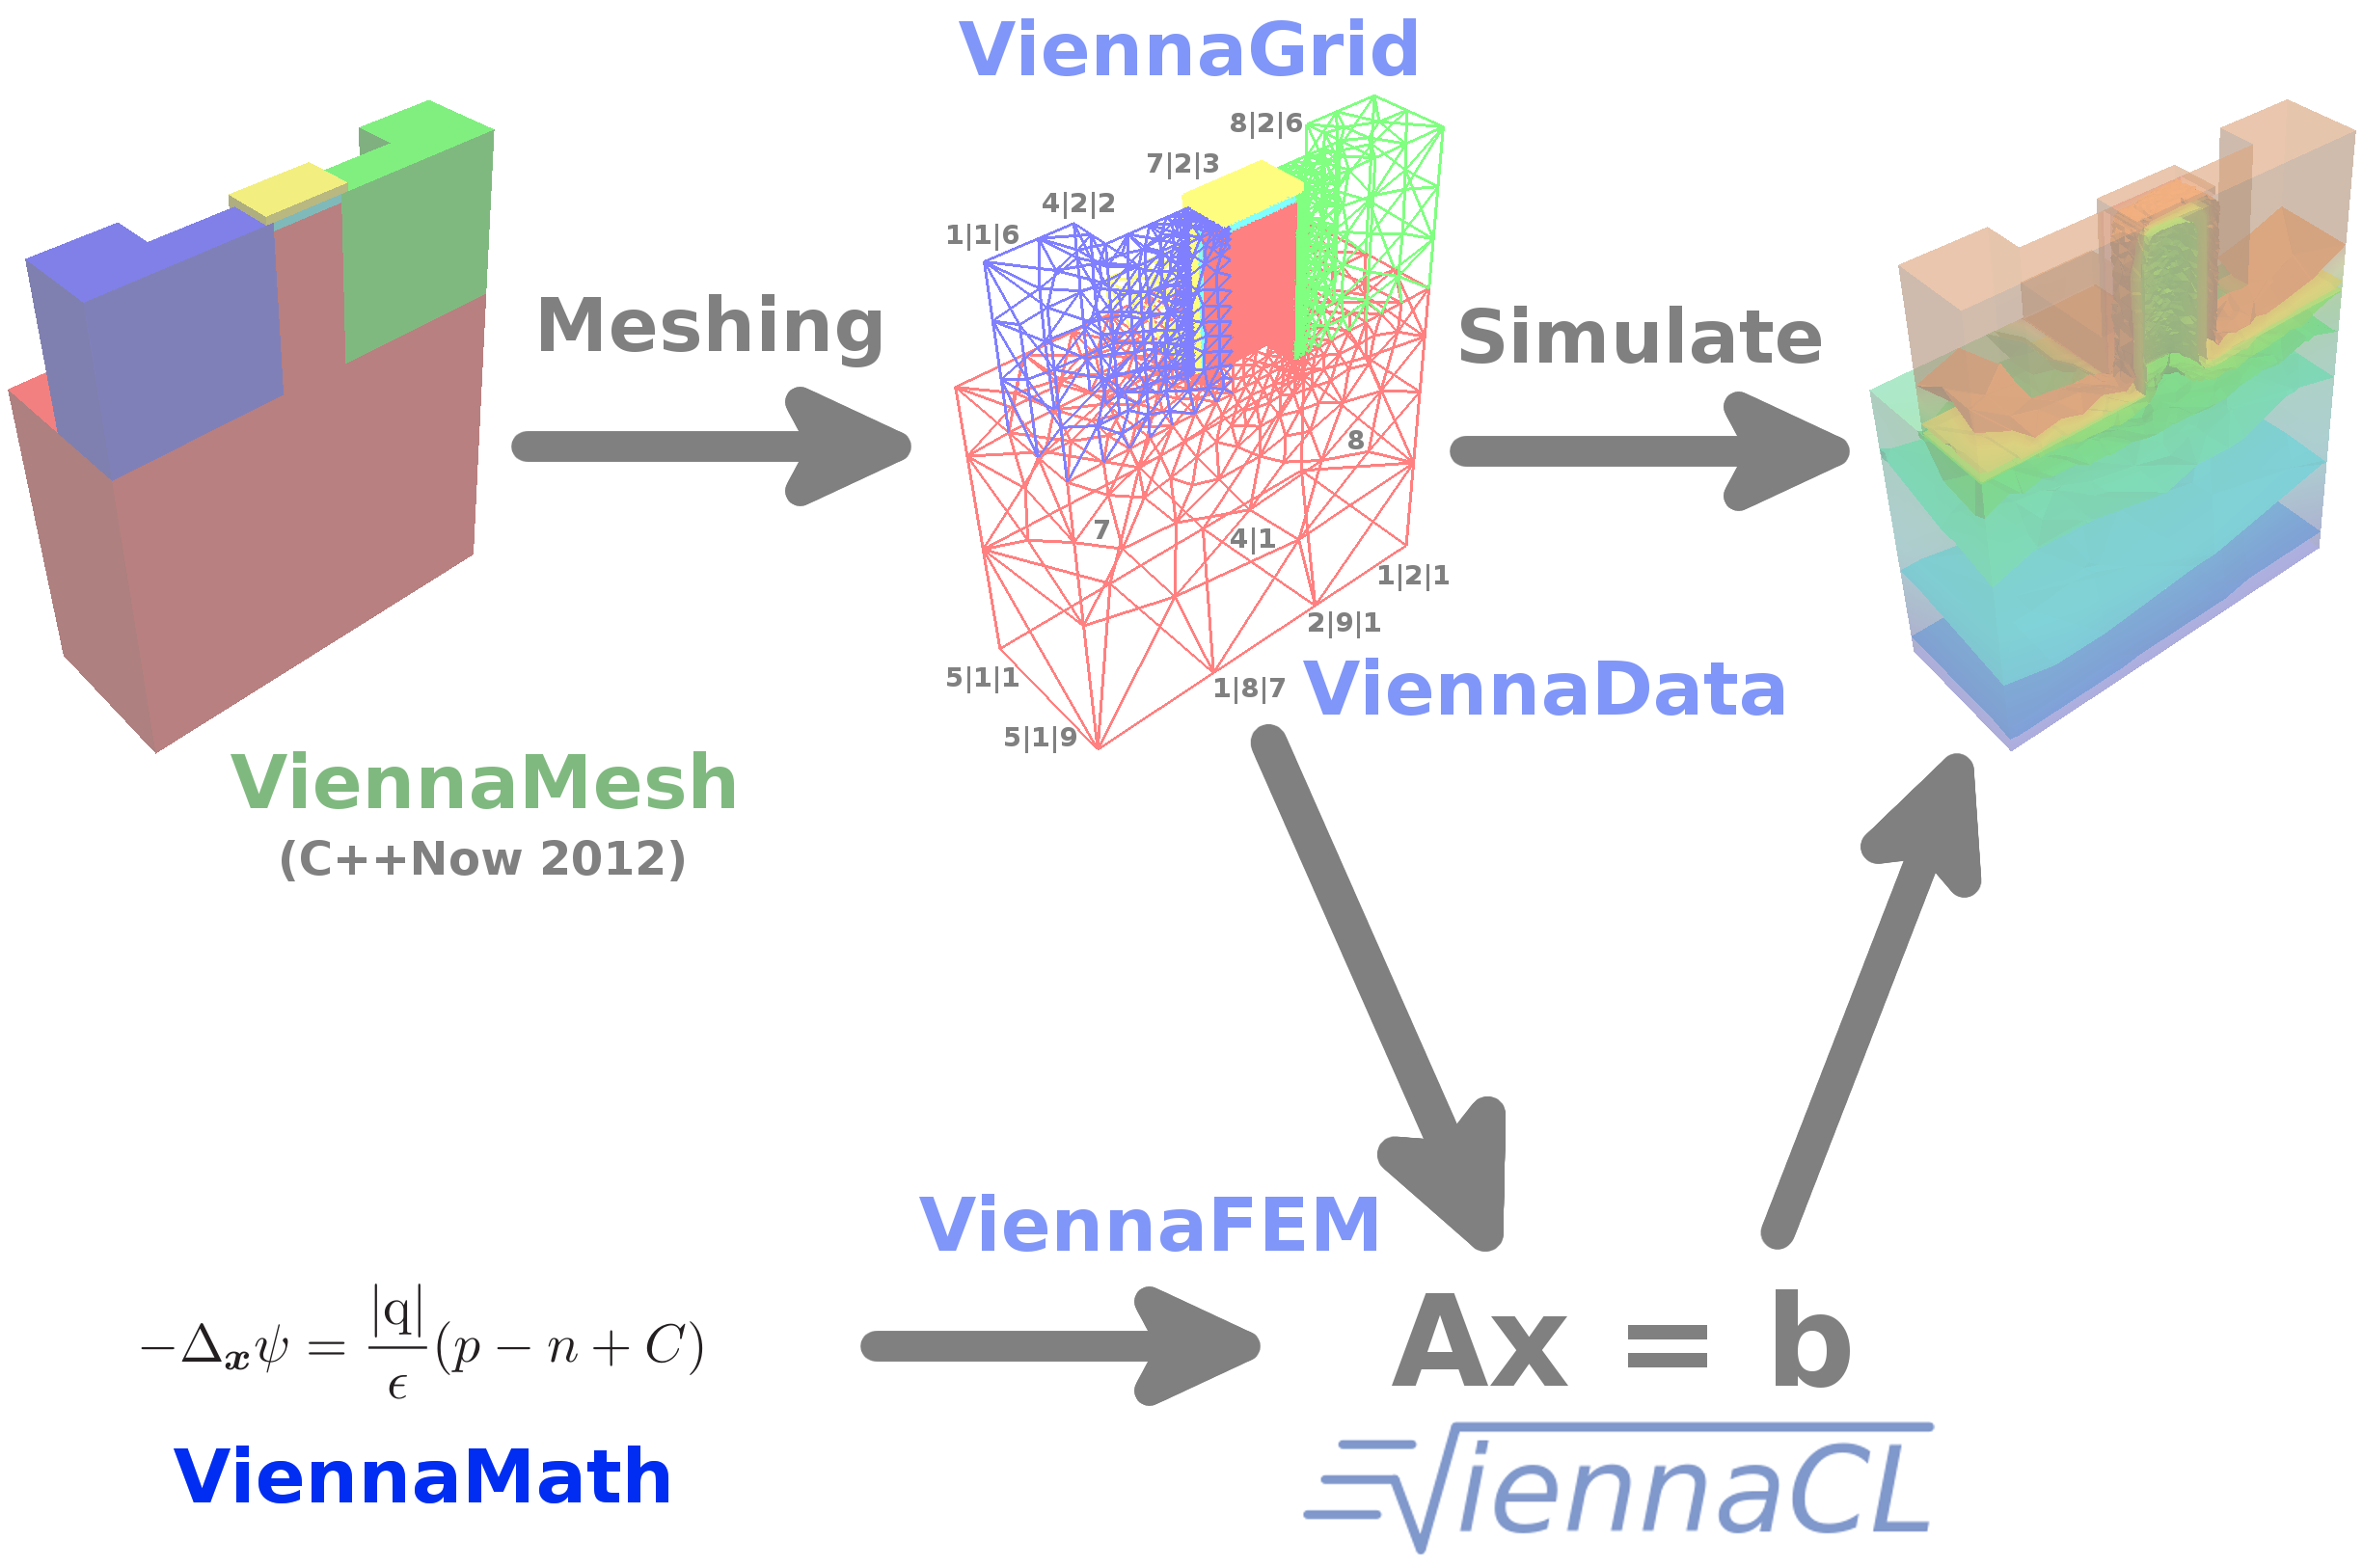
\includegraphics[width=0.99\textwidth]{flow-viennamath-2.png}
  \end{center}
\end{frame}


%%%%%% Expected talk time: 15 minutes, ~7 slides



\begin{frame}[fragile]
\frametitle{ViennaMath}

 \begin{block}{A Symbolic Math Library in C++}
   \begin{itemize}
    \item Symbolic evaluation and manipulation of math expressions
    \item Unified run time and compile time interface
    \item Differentiation and integration provided
    \item {\LaTeX} output
   \end{itemize}
 \end{block}

 \begin{block}{Example Usage}
\begin{lstlisting}
  variable x(0);
  variable y(1);
  variable z(2);
  expr f = x + y - z;
  expr g = f * f;
  eval(f, make_vector(1.0, 2.0, 4.0)); // returns -1.0
  eval(g, make_vector(1.0, 2.0, 4.0)); // returns  1.0
\end{lstlisting} 
   \begin{itemize}
    \item Run Time Evaluation
   \end{itemize}
 \end{block}
\end{frame}



%%%%%%%%%%%%%%%%%%%%%

\begin{frame}[fragile]
\frametitle{ViennaMath}

 \begin{block}{A Symbolic Math Library in C++}
   \begin{itemize}
    \item Symbolic evaluation and manipulation of math expressions
    \item Unified run time and compile time interface
    \item Differentiation and integration provided
    \item {\LaTeX} output
   \end{itemize}
 \end{block}

 \begin{block}{Example Usage}
\begin{lstlisting}
  ct_variable<0> x;
  ct_variable<1> y;
  ct_variable<2> z;
  ct_constant<1> c1;
  ct_constant<2> c2;
  ct_constant<4> c4;
  eval(x + y - z, make_vector(c1, c2, c4)); // returns -1
\end{lstlisting} 
   \begin{itemize}
    \item Compile Time Evaluation
   \end{itemize}
   \vspace*{-0.05cm}
 \end{block}
\end{frame}

%%%%%%%%%%%%%%%%%%%%%%%%%%%%%%%%%



\begin{frame}[fragile]
\frametitle{ViennaMath}

 \begin{block}{Substitution and Differentiation (Run Time)}
\begin{lstlisting}
  variable x(0);
  variable y(1);
  variable z(2);
  substitute(x, y, x*y + z); // returns y*y+z
  diff(x*y + z, x);          // returns y
\end{lstlisting} 
 \end{block}
 
 \begin{block}{Substitution and Differentiation (Compile Time)}
\begin{lstlisting}
  ct_variable<0> x;
  ct_variable<1> y;
  ct_variable<2> z;
  substitute(x, y, x*y + z); // returns y*y+z
  diff(x*y + z, x);          // returns y
\end{lstlisting} 
 \end{block}
 
\end{frame}

%%%%%%%%%%%%%%%%%%%%%%%%%%%%%%%%


\begin{frame}[fragile]
\frametitle{ViennaMath}

 \begin{block}{Numerical Integration (Run Time): $\color{black} \int_0^1 x^2 \: \mathrm{d} x$}
\begin{lstlisting}
  expr f = integral( make_interval(0, 1), x*x, x );

  numerical_quadrature integrator(new gauss_quad_1());
  integrator(f);                             // method 1
  integrator(make_interval(0, 1), x*x, x);   // method 2
\end{lstlisting} 
 \end{block}
 
 \begin{block}{Analytical Integration (Compile Time): {\color{black} $\int_0^1 x^2 \: \mathrm{d} x$, $\int_0^1 \int_0^{1-x} xy \: \mathrm{d}x \mathrm{d}y$} }
\begin{lstlisting}
  integrate(make_interval(c0, c1),
            x*y,
            x );    //returns y/2.0
  integrate(make_interval(c0, c1),
            integrate( make_interval(c0, c1 - x), x*y, y),
            x);    //returns 1.0/24.0
\end{lstlisting} 
 \end{block}
 
\end{frame}

%%%%%%%%%%%%%%%%%%%%%%%%%%%%%%%%


\begin{frame}[fragile]
\frametitle{ViennaMath}

 \begin{block}{Function Symbols}
   \begin{itemize}
    \item Represent a function (not evaluable)
   \end{itemize}
 \end{block}

 \begin{block}{Differential Operators}
   \begin{itemize}
    \item Gradient, Divergence
   \end{itemize}
 \end{block}

 \begin{block}{Symbolic Integration Domain}
   \begin{itemize}
    \item Specify actual integration domain and integration variables \emph{later}
   \end{itemize}
 \end{block}
 
\begin{lstlisting}
  function_symbol u;
  equation eq( laplace(u), 1.0 );  // Poisson equation
  
  function_symbol v;
  expr w = integral(symbolic_interval(),
                    grad(u) * grad(v));
\end{lstlisting} 
 
\end{frame}



% Maybe throw in one or two more slides


